\chapter{Function}
\begin{table}[ht]
\centering
    \begin{tabular}{ | l | p{5.5cm} | p{5cm} |}
    \hline
    Function  & File Use & Summary \\ \hline
    \texttt{millis} & \texttt{RADIO} \newline
    \texttt{base\_station} \texttt{customer\_premise\_equipment} \texttt{licensed\_band\_user} & extracts current time based on internal clock. \\ \hline
    \texttt{random} & \texttt{base\_station} & generates random integers for a given range. \\ \hline
    \texttt{delay} & \texttt{TEST} \newline
    \texttt{base\_station} \texttt{customer\_premise\_equipment} \texttt{licensed\_band\_user} & waits for a given time ms. \\\hline
    \texttt{digitalWrite} & \texttt{base\_station} \texttt{customer\_premise\_equipment} & sets a out put pin to a voltage value. \\\hline
    \texttt{pinMode} & \texttt{base\_station} \texttt{customer\_premise\_equipment} \texttt{licensed\_band\_user} & specifies digital GPIO usage.\\\hline
    \texttt{Serial.begin} & \texttt{base\_station} \texttt{customer\_premise\_equipment} \texttt{licensed\_band\_user} & initializes serial ports baud rate. \\\hline
    \texttt{Serial.print} & \texttt{base\_station} \texttt{customer\_premise\_equipment} \texttt{licensed\_band\_user} & output data to monitor through serial ports. \\\hline
    \hline
    \end{tabular}
\caption{Functions used from \texttt{Arduino}}
\label{tab:function}
\end{table}

\leavevmode\newline

\begin{table}[ht]
\centering
    \begin{tabular}{ | l | p{5.5cm} | p{6cm} |}
    \hline
    Function  & File Use & Summary \\ \hline
    \texttt{read} & \texttt{TEST} & reads the value in a given memory location. \\ \hline
    \texttt{write} & \texttt{TEST} & writes the value into a given memory location. \\ \hline
    \hline
    \end{tabular}
\caption{Functions used from \texttt{EEPROM}}
\label{tab:function2}
\end{table}

\leavevmode\newline

\begin{ThreePartTable}
\begin{TableNotes}
\footnotesize
\item Note: This table concludes all the functions used by \texttt{RADIO} to develop more handy subroutine for the system.
\end{TableNotes}
\begin{longtable}[ht]{ | l | p{10cm} | {c}}
\caption{Functions in \texttt{ELECHOUSE\_CC1101\_SRC\_DRV}}  \\
\hline
    Function & Summary \\ \hline
    \texttt{Init} & presets module registers. Each device must be set to initialize the cc1101. \\ \hline
    \texttt{setCCMode} & sets configuration for internal transmission mode. \\ \hline
    \texttt{setModulation} & sets modulation mode. 0 = 2-FSK, 1 = GFSK, 2 = ASK/OOK, 3 = 4-FSK, 4 = MSK. \\\hline
    \texttt{setMHz} & sets the basic frequency. The lib calculates the frequency automatically (default = 433.92).The cc1101 can: 300-348 MHZ, 387-464MHZ and 779-928MHZ. Read More info from datasheet. \\\hline
    \texttt{setDeviation} & sets the frequency deviation in kHz. Value from 1.58 to 380.85. Default is 47.60 kHz.\\\hline
    \texttt{setChannel} & sets the Channel number from 0 to 255. Default is channel 0. \\\hline
    \texttt{setChsp} & sets to multiply by the channel number CHAN and added to the base frequency in kHz. Value from 25.39 to 405.45. Default is 199.95 kHz. \\\hline
    \texttt{setRxBW} & sets the Receive Bandwidth in kHz. Value from 58.03 to 812.50. Default is 812.50 kHz. \\\hline
    \texttt{setDRate} & sets the Data Rate in kBaud. Value from 0.02 to 1621.83. Default is 99.97 kBaud. \\\hline
    \texttt{setPA} & sets TxPower. The following settings are possible depending on the frequency band.  (-30  -20  -15  -10  -6    0    5    7    10   11   12) Default is max! \\\hline
    \texttt{setSyncMode} & combines sync-word qualifier mode. 0 = No preamble/sync. 1 = 16 sync word bits detected. 2 = 16/16 sync word bits detected. 3 = 30/32 sync word bits detected. 4 = No preamble/sync, carrier-sense above threshold. 5 = 15/16 + carrier-sense above threshold. 6 = 16/16 + carrier-sense above threshold. 7 = 30/32 + carrier-sense above threshold. \\\hline
    \texttt{setSyncWord} & sets sync word. Must be the same for the transmitter and receiver. (Syncword high, Syncword low) \\\hline
    \texttt{setAdrChk} & controls address check configuration of received packages. 0 = No address check. 1 = Address check, no broadcast. 2 = Address check and 0 (0x00) broadcast. 3 = Address check and 0 (0x00) and 255 (0xFF) broadcast. \\\hline
    \texttt{setAddr} & modifies address used for packet filtration. Optional broadcast addresses are 0 (0x00) and 255 (0xFF). \\\hline
    \texttt{setWhiteData} & turns data whitening on / off. 0 = Whitening off. 1 = Whitening on. \\\hline
    \texttt{setPktFormat} & formats RX and TX data. 0 = Normal mode, use FIFOs for RX and TX. 1 = Synchronous serial mode, Data in on GDO0 and data out on either of the GDOx pins. 2 = Random TX mode; sends random data using PN9 generator. Used for test. Works as normal mode, setting 0 (00), in RX. 3 = Asynchronous serial mode, Data in on GDO0 and data out on either of the GDOx pins. \\\hline
    \texttt{setLengthConfig} & sets the length of message. 0 = Fixed packet length mode. 1 = Variable packet length mode. 2 = Infinite packet length mode. 3 = Reserved \\\hline
    \texttt{setPacketLength} & indicates the packet length when fixed packet length mode is enabled. If variable packet length mode is used, this value indicates the maximum packet length allowed. \\\hline
    \texttt{setCrc} & chooses CRC option. 1 = CRC calculation in TX and CRC check in RX enabled. 0 = CRC disabled for TX and RX. \\\hline
    \texttt{setCRC\_AF} & Enable automatic flush of RX FIFO when CRC is not OK. This requires that only one packet is in the RXIFIFO and that packet length is limited to the RX FIFO size. \\\hline
    \texttt{setDcFilterOff} & disables digital DC blocking filter before demodulator. Only for data rates less than or equal to 250 kBaud The recommended IF frequency changes when the DC blocking is disabled. 1 = Disable (current optimized). 0 = Enable (better sensitivity). \\\hline
    \texttt{setManchester} & enables Manchester encoding/decoding. 0 = Disable. 1 = Enable. \\\hline
    \texttt{setFEC} & enables Forward Error Correction (FEC) with interleaving for packet payload (Only supported for fixed packet length mode. 0 = Disable. 1 = Enable. \\\hline
    \texttt{setPQT} & sets the preamble quality estimator threshold. The preamble quality estimator increases an internal counter by one each time a bit is received that is different from the previous bit, and decreases the counter by 8 each time a bit is received that is the same as the last bit. A threshold of 4 PQT for this counter is used to gate sync word detection. When PQT=0 a sync word is always accepted. \\\hline
    \texttt{setAppendStatus} & enables status with two bytes be appended to the payload of the packet. The status bytes contain RSSI and LQI values, as well as CRC OK. \\\hline
    \texttt{CheckRxFifo} & checks if the receive flag is raised, buffer then ready to receive data\\\hline
    \texttt{CheckCRC} & uses cyclic redundancy check to ensure fullness of the data \\\hline
    \texttt{ReceiveData} & puts data to a buffer  \\\hline
    \texttt{SendData} & send data from the buffer to the air \\\hline
    \insertTableNotes  % tell LaTeX where to insert the contents of "TableNotes"
%\caption*{State Table for the proposed network (continued)}\\
\label{tab:function3}
\end{longtable}
\end{ThreePartTable}

\begin{table}[ht]
\centering
    \begin{tabular}{ | l | l | l | l | l | p{4cm} |}
    \hline
    Operation & opcode & payload & src & dest & Summary \\ \hline
    cpeRequest & 1 & T$^a$  & requester$^b$  & receiver$^c$ & sends whenever the requesting CPE wants to set up a connection with another CPE \\ \hline
    cpeRespond & 2 & CH$^d$ & receiver & requester & responds back to the requesting CPE by confirming the channel\\ \hline
    cpeSend & 3 & X$^e$ & receiver & requester & sends to the receiving CPE at the assigned channel \\ \hline
    bsRequest & 5 & CH & requester & receiver & forwards the message to the target CPE with BS selected channel\\ \hline
    bsRespond & 6 & CH & receiver & requester & forwards the response from the target CPE back to the requesting CPE\\ \hline
    cpeStart & 7 & X & requester & X & initiates the CPE initial connection to the BS\\ \hline
    lbuInterrupt & 8 & X & X & X & sends to interrupt the CPE communications \\ \hline
    lbuStart & 11 & X & requester & X & initiates the LBU initial connection to the BS \\ \hline
    bsStart & 12 & X & X & X & broadcasts to finish the synchronization process\\ \hline
    \hline
    \end{tabular}
\footnotesize{
$^a$ The varying communication time duration \
$^b$ The device that initiates the connection 
$^c$ The device that would catch the message 
$^e$ The assigned channel 
$^e$ Representation of a Don't Care value}\\
\caption{Message structure}
\label{tab:structure}
\end{table}


\chapter{Specification}

\begin{table}[ht]
\centering
    \begin{tabular}{ | p{5cm} | p{8cm} |}
    \hline
    Microcontroller & ATmega328\\ \hline
    Architecture & AVR\\ \hline
    Operating Voltage & 5 V\\ \hline
    Flash Memory & 32 KB of which 2 KB used by bootloader\\ \hline
    SRAM & 2 KB\\ \hline
    Clock Speed & 16 MHz\\ \hline
    Analog IN Pins & 8\\ \hline
    EEPROM & 1 KB\\ \hline
    DC Current per I/O Pins & 40 mA (I/O Pins)\\ \hline
    Input Voltage & 7-12 V\\ \hline
    Digital I/O Pins & 22 (6 of which are PWM)\\ \hline
    PWM Output & 6\\ \hline
    Power Consumption & 19 mA\\ \hline
    PCB Size & 18 x 45 mm\\ \hline
    Weight & 7 g\\ \hline
    Product Code & A000005\\ \hline
    \hline
    \end{tabular}
\caption{Arduino Nano Specification}
\label{tab:arduino_spec} \cite{arduino_nano}
\end{table}

\begin{table}[ht]
\centering
    \begin{tabular}{ | p{2cm} | p{5cm} | p{7cm} |}
    \hline
    No. & Parameter item & Parameter details and description\\ \hline
    1 & Size & 15 * 30mm\\ \hline
    2 & Components & Imported from Japan, USA and Germany\\ \hline
    3 & Connector & 2*4*2.54mm\\ \hline
    4 & Supply voltage & 1.9 - 3.6V DC (Notes: the voltage higher than 3.6V is forbidden.)\\ \hline
    5 & Frequency Band & 387 - 464MHz, adjustable, Recommending frequency: 433±10MHz\\ \hline
    6 & Communication level & 0.7VCC - 3.6V (VCC refers to the supply voltage)\\ \hline
    7 & Operation Range & About 520m(test condition: clear and open area and maximum power, antenna gain: 5dBi, height: $>$ 2m, air date rate:     1.2Kbps)\\ \hline
    8 & Transmitting power & Maximum 10dbm (10mW)\\ \hline
    9 & Air data rate & 0.6k - 500k(1.2~20kbps is recommended)\\ \hline
    10 & Sleep current & 0.6uA\\ \hline
    11 & Transmitting current & 29.2mA at 10dBm\\ \hline
    12 & Receiving current & 16.0mA  \\ \hline
    13 & Communication interface & SPI (data rate: up to 10Mbps)\\ \hline
    14 & Transmitting length & 1 - 64 bytes for one package\\ \hline
    15 & Receiving length & 1 - 64 bytes for one package\\ \hline
    16 & RSSI support & usable\\ \hline
    17 & Antenna type & SMA-K(External thread hole, 50 ohm impedance)\\ \hline
    18 & Sensitivity & -116dBm at 0.6kbps, -112dBm at 1.2kbps\\ \hline
    19 & Operating temperature & -40 \textasciitilde +85\textdegree{}C \\ \hline
    20 & Operating humidity & 10\% ~ 90\%\\ \hline
    21 & Storage temperature & -40 \textasciitilde +125\textdegree{}C \\ \hline
    \hline
    \end{tabular}
\caption{CC1101 Module Specification}
\label{tab:cc1101_spec}\cite{cc1101_module}
\end{table}


\chapter{Bill Of Material}
\begin{table}[h]
\centering
    \begin{tabular}{| l | l | l | c | r | }
    \hline
    Item & Description & Quantity & Units & Cost \\ 
    \hline
    \rowcolor{lightgray} Arduino Nano & MCU ATmega328 & 1 &  Dozen &  50.16 \\ 
    Arduino Adaptor  &  3.0 USB to mini USB & 1 &  Each &  0.64 \\ 
    \rowcolor{lightgray} Transceiver Module & E07-M1101D Board V2.0 & 1 &  Dozen &  33.6 \\ 
    Level Shifter &  pack of 10 & 2 &  Package & 13.98 \\ 
    \rowcolor{lightgray} Pin Header Socket &  16, 6 and 4 pins, pack of 10 & 12 &  Package &  5.76 \\ 
    Prototype Board & 5 x 7cm, pack of 10 & 1 &  Package &  4 \\ 
    \rowcolor{lightgray} Battery & 9V & 10 & Each &  1 \\ 
    Battery Connector &  T type Battery Connector & 1 & Dozen & 1.3 \\ 
    \rowcolor{lightgray} Light-emitting Diode &  blue and yellow & 20 &  Each &  1.04 \\ 
    Wire &  3m roll & 2 & Each &  1 \\ 
    \rowcolor{lightgray} Solder &  solder wire roll, 50g, 1mm & 3 &  Each &  1.71 \\ 
    \hline
    \hline
    \end{tabular}
    \begin{tablenotes}
    \small
    \item Note: The necessary tools such as the IDE accessible client machine or soldering iron are not included here.
\end{tablenotes}
\caption{Bill of Material}
\label{tab:bill}
\end{table}

\chapter{Simulink}
\begin{figure}[ht]
\centering
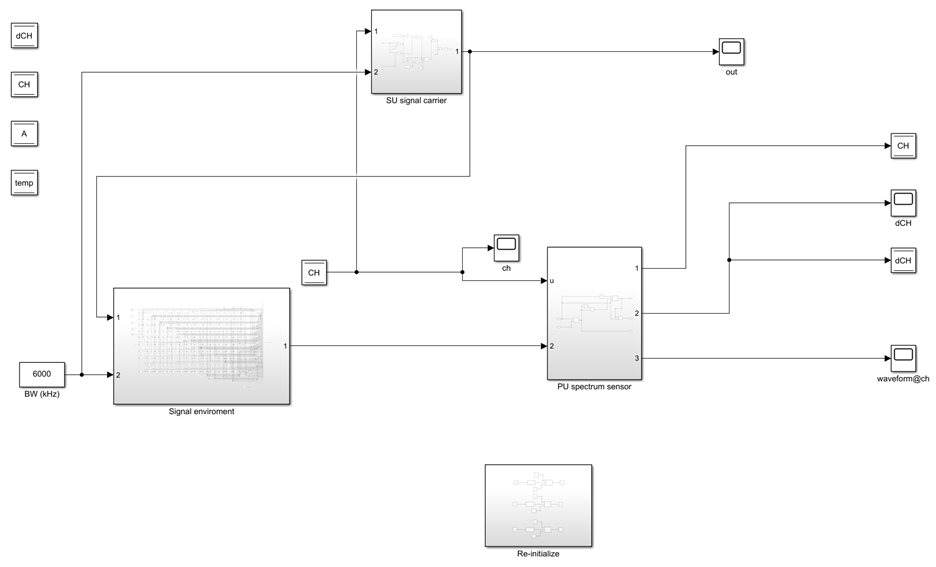
\includegraphics[width=12cm]{figures/top_level_simulink.png}
\caption{Top Level Block}
\label{fig:top_level_simulink}
\end{figure}

\begin{figure}[ht]
\centering
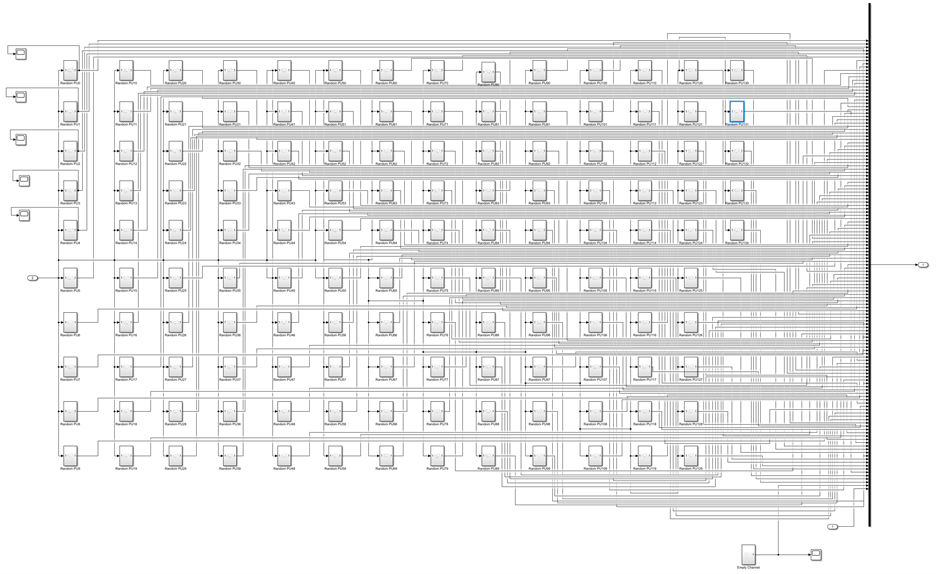
\includegraphics[width=12cm]{figures/random_signal_simulink.png}
\caption{Random Signal Generator Block}
\label{fig:random_signal_simulink}
\end{figure}

\chapter{Python Simulation}
\begin{lstlisting}[caption={Selected main process code in Python simulation},captionpos=b]
# Available at
# https://github.com/SaltFishBoi/cognitive_radio_network_simulator 
from base_station import *
from customer_premise_equipment import *
from licensed_band_user import *
from transmission import *
from algorithm import *
from multiprocessing import Process
import time

INTERRUPT_FLAG = 0

def main():

    # initialize environment channel list
    share_env1 = create_environment()

    # initialize base station
    bs = BS(0)

    # CPE action list
    # actions list (EDITABLE)
    # (delay, target)
    action_list = [[ACTION(1, 1, 10), ACTION(1, 11, 10)],
                   [ACTION(2, 2, 10), ACTION(2, 12, 10)],
                   [ACTION(3, 3, 10), ACTION(3, 13, 10)],
                   [ACTION(4, 4, 10), ACTION(4, 14, 10)],
                   [ACTION(5, 5, 10), ACTION(5, 15, 10)],
                   [ACTION(6, 6, 10), ACTION(6, 16, 10)],
                   [ACTION(1, 7, 10), ACTION(1, 17, 10)]]

    schedule_list = [[6, 6, 7, 8, 9],
                     [6, 6, 7, 8, 9],
                     [6, 6, 7, 8, 9],
                     [6, 6, 7, 8, 9],
                     [6, 6, 7, 8, 9],
                     [6, 6, 7, 8, 9],
                     [6, 6, 7, 8, 9],
                     [6, 6, 7, 8, 9],
                     [6, 6, 7, 8, 9],
                     [6, 6, 7, 8, 9],
                     [6, 6, 7, 8, 9]]

    print("Program Starts")

    # launch multiprocess

    t = Process(target=timing)
    t.start()

    b = Process(target=bs_process, args=(share_env1, bs))
    print("Program runs")
    cpe_proc = []
    lbu_proc = []
    b.start()

    # initialize and launch license band user list
    for i in range(1, NUM_LBU_DEFAULT+1):
        device = LBU(i, STATE_DEFAULT, i)
        l = Process(target=lbu_process, args=(share_env1, i, device, schedule_list[i-1]))
        l.start()
        lbu_proc.append(l)

    # initialize and launch customer premise equipment list
    for i in range(NUM_CPE_DEFAULT):
        device = CPE(i)
        c = Process(target=cpe_process, args=(share_env1, i, device, action_list[i]))
        c.start()
        cpe_proc.append(c)

    # recycle all processes
    for c in cpe_proc:
        c.join()

    for l in lbu_proc:
        l.join()

    b.join()
    t.join()
    print("Program ends")

    return 0

def timing():
    i = 0
    while True:
        print("    Time: ", i)
        time.sleep(1)
        i += 1
        
# Press the green button in the gutter to run the script.
if __name__ == '__main__':
    #stdoutOrigin = sys.stdout
    #sys.stdout = open("log.txt", "w")
    main()
\end{lstlisting}



